
\chapter{Speaker Recognition in Co-channel Speech}
\label{chapter:backend}

%\begin{figure}[b]
%	\hrule
%	\vspace{.03cm}
%	{\rmfamily{\small \em { Mail All Correspondence To:}\vspace{-0.2cm}\\}}
%	\begin{minipage}{0.2\linewidth}
%		\centering
%		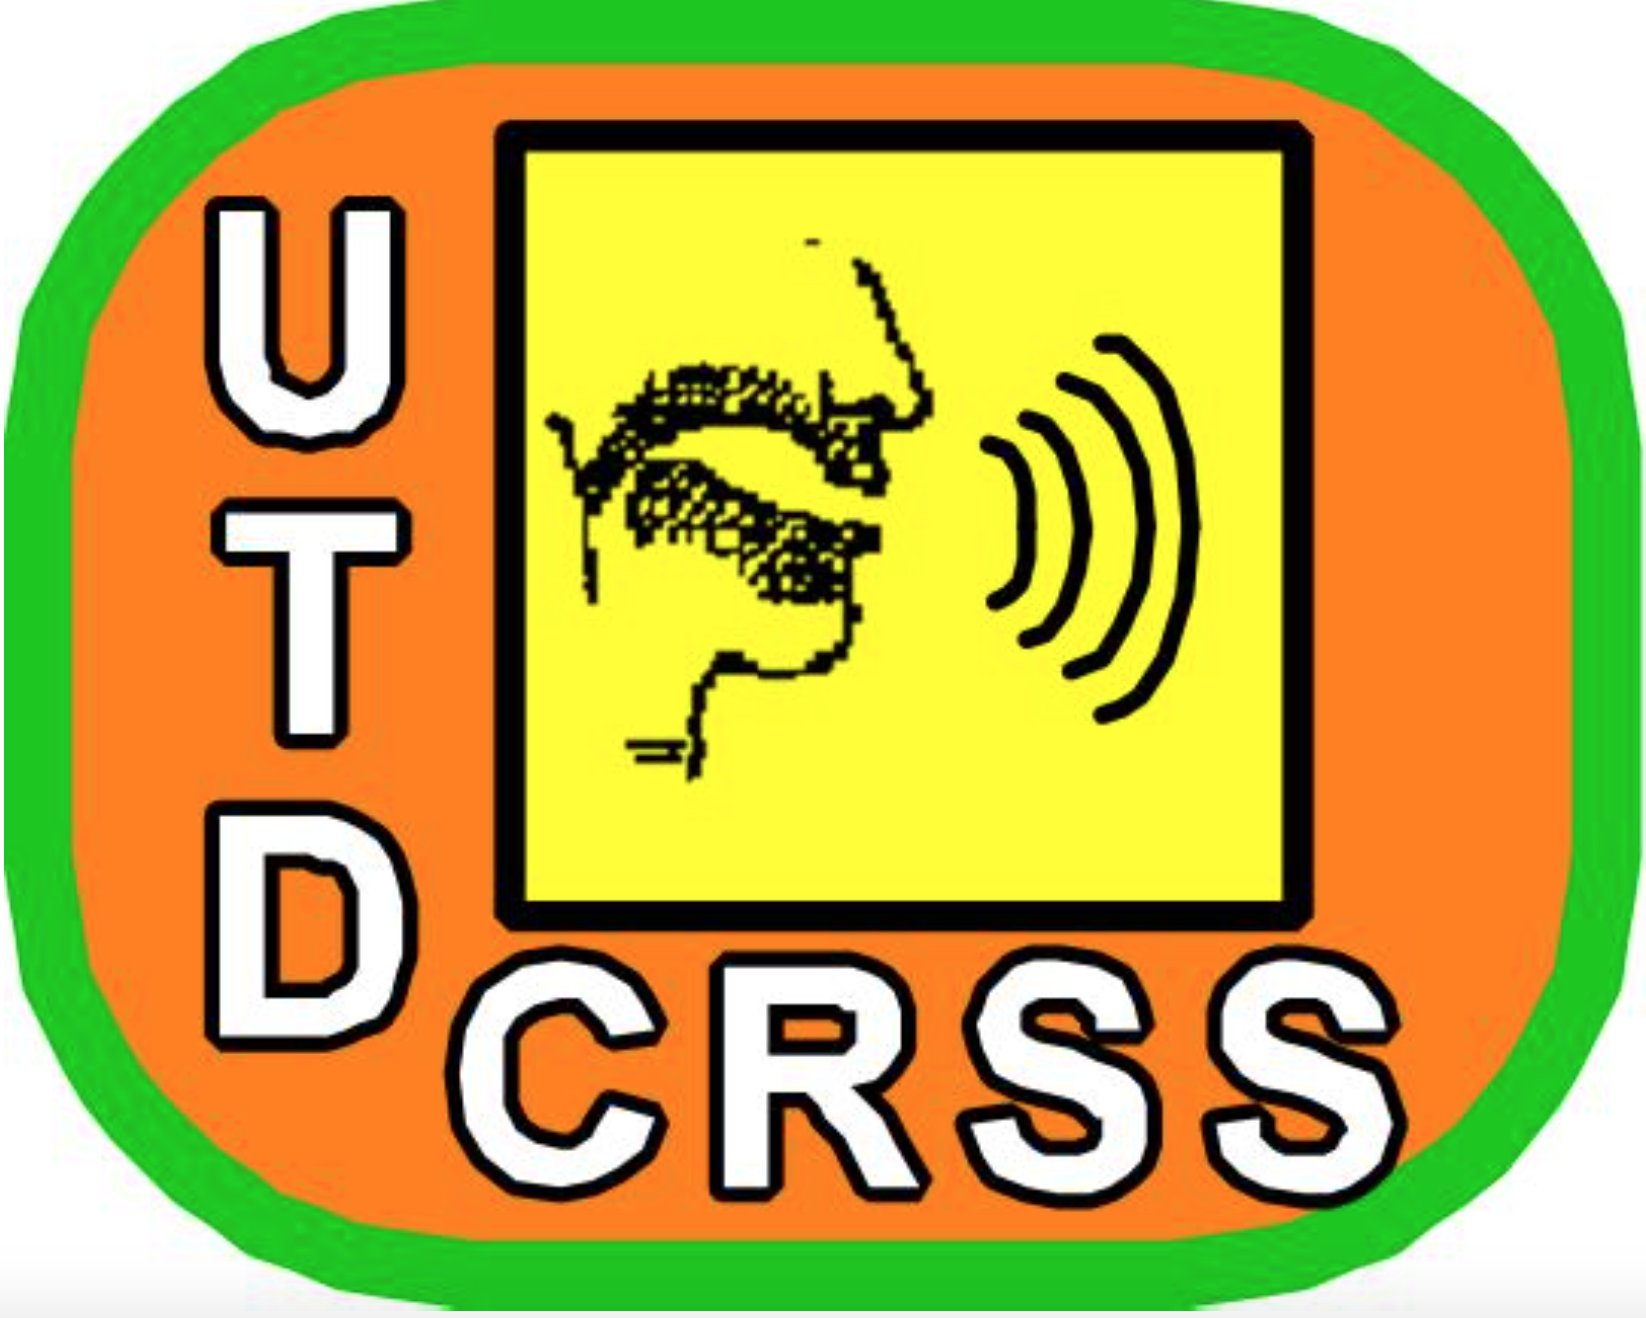
\includegraphics[width=1\linewidth]{chapters/cochannelplda_jp/IEEEtran/figures/CRSS_logo}
%	\end{minipage}
%	\begin{minipage}{0.8\linewidth}
%		\begin{singlespace}
%			\small \vspace{.5cm}
%			\footnotesize
%			Prof. John H.L. Hansen\\
%			Center for Robust Speech Systems (CRSS), Erik Jonsson School of Engineering and Computer Science, Dept. of
%			Electrical Engineering, University of Texas at Dallas\\
%			2601 N. Floyd Road, EC33, Richardson, TX 75080-1407, U.S.A\\
%		\end{singlespace}
%	\end{minipage}
%	\small{$^*$This project was funded by AFRL under contract FA8750-12-1-0188 and partially by the University of Texas at Dallas from the Distinguished University Chair in Telecommunications Engineering held by J.H.L. Hansen.}\\
%\end{figure}

This chapter addresses the problem of speaker recognition for co-channel recordings, rather than speaker recognition in overlap. 
The main focus is on interference from secondary speakers, be it overlapped or not. 
Secondary speech interference, the main characteristic of co-channel, is an important source of error for all automatic speech processing systems. Speaker recognition experiments are highly influenced by the presence of secondary speakers, due to reduced reliability of the trained models. 
Although the target speaker is a common factor in all training samples for a given speaker model, the standard structure of speaker recognition systems has not been designed to average out interfering speech. 

To the best of our knowledge, few studies address speaker recognition in co-channel speech signals. 
However, the effects of artificially adding {\bf overlapped speech} in a speaker verification setup has received considerable attention~\cite{yantorno_report,yantorno_SID,Dwang_03}. 
In many of these studies, the approach was to automatically detect and remove overlaps from co-channel speech in training and test data. 
Although many overlap detection algorithms have been investigated over the years~\cite{Boakye_icassp_08,nav_icassp13,smolenski_tut,sapvr_2000}, none have considered solving the problem in the more general case of co-channel interference. 

This chapter differentiates co-channel speech from overlapped speech by considering the latter a special case of the former where both speakers are active at the same time. 
Co-channel speech refers to the broader case where speakers are not necessarily overlapping (see Fig.~\ref{fig:cochannel_vs_overlap}). 
We focus on speaker recognition in co-channel speech interference, in which overlaps may occur.  
This sheds light on a more realistic problem, since only a small percentage of conversational speech contains amounts of overlap that are large enough to significantly lower speaker recognition performance~\cite{cetin_shriberg_06_icassp,smolenski_tut}. 

\begin{figure*}[t!]
	\centering
	\vspace{0mm}
	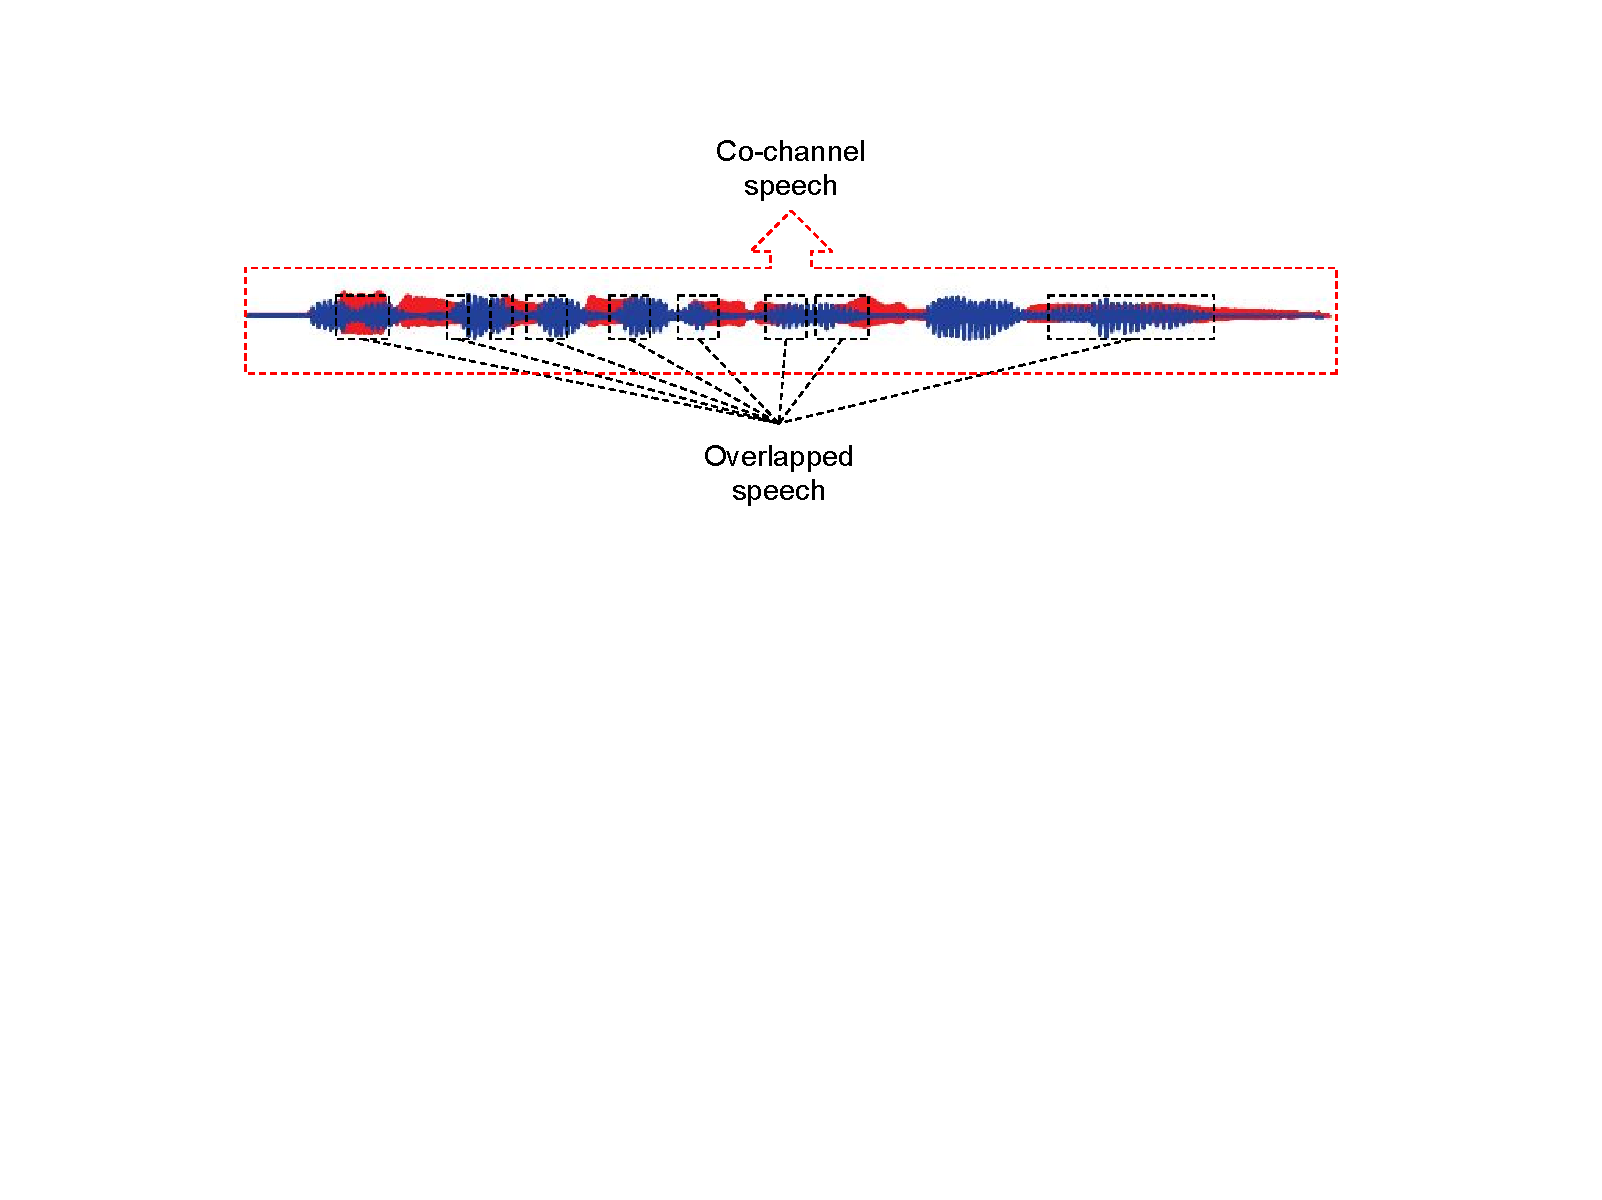
\includegraphics[height = 2in, width=0.9\textwidth]{figures/cochannel_vs_overlap-crop}
	\vspace{-3mm}
	\caption{\it \small Difference between co-channel and overlapped speech. Overlap refers to instances where more than one speaker is active. Co-channel is defined as an entire stream that contains multiple speakers. All co-channel files do not necessarily contain overlap. }
	\label{fig:cochannel_vs_overlap}
	\vspace{-3mm}
\end{figure*}


A commonsense solution to co-channel interference for speaker recognition, would be to separate speech from unwanted speakers from the original signal. 
The difference between what we present here and existing studies in speaker recognition for co-channel speech is that we would like to bypass solutions that require removing interfering speech from the original signal. 
Such solutions are primarily known as speaker diarization. 
Speaker diarization is defined as the task of determining ``who spoke when?'' within an audio recording. 
Using diarization as a preprocessing step for speaker recognition in co-channel speech involves determining speaker identities in short segments within each recording, a task which is itself a speaker recognition problem.  
Alternatively, we are interested in modifying model parameters extracted from co-channel data in a way that would only represent the primary speaker. 

The solution we would like to focus on in this chapter is a model-based approach, rather than signal-based (e.g. speaker diarization). 
Currently, the most common form of modeling speaker-dependent features are i-vectors~\cite{dehak2011front}. 
I-vectors are latent parameters that model the covariance of speaker/session-dependent Gaussian mixture models (GMM) with respect to a generic GMM (aka Universal background model -- UBM).  
The UBM is ideally both session- and speaker-independent.
The use of i-vectors, has become a standard way of modeling speaker specific traits for speaker recognition. 
In many cases i-vector extraction is considered a preprocessing step in performing speaker recognition\footnote{See Appendix~\ref{apndx:spkr_id}}. 
Therefore, it is both reasonable and desirable to concentrate on post i-vector analysis to deal with co-channel speech interference~\cite{ivector_challenge}. 
The goal of this study is to build upon the latent variable perspective, popularized by i-vectors~\cite{dehak2011front} and its predecessors~\cite{kenny2010bayesian}, to improve speaker recognition in co-channel signals. 
Working in the latent variable subspace provides the luxury of short-circuiting speaker diarization, a computationally intensive and potentially error-prone solution. 


To further refine our problem statement, the following ground rules are set. We assume that: 1) Sufficient data is available from multiple recording sessions to train speakers. 
2) Co-channel data is used in the evaluation set. In the standard i-vector speaker recognition framework, often a number of recordings are provided for each speaker. 
These i-vectors can then be projected onto a subspace using probabilistic linear discriminant analysis (PLDA)~\cite{prince_plda} to compensate for channel variations\footnote{Channel variation refers to differences in recording conditions and devices. The authors feel obligated to remind readers not to confuse channel information with co-channel speech.} across different recordings~\cite{kenny_plda,Daniel2011is}. 
Therefore, latent variables in the PLDA subspace are calculated in a way to only represent speaker-dependent information~\cite{kenny_plda2,cumani_icassp13,burget_icassp11,yun_icassp12}.
Now if i-vectors are to be extracted from co-channel signals, the speaker-dependent latent variables from PLDA must represent a combination of all speakers in the original audio file. 
In the case of speaker recognition in co-channel speech, the task of our proposed system would be to also account for the fact that i-vectors might have been extracted from co-channel sessions. 

We investigate using modified versions of the PLDA paradigm to make i-vectors collected from co-channel sessions suitable for speaker recognition experiments. The goal is to create overall robustness with respect to interfering speech. 
PLDA uses inter- and intra-session variabilities from a development set to find a subspace in the i-vector space that best represents speaker dependencies. 
Here we investigate the possibility of performing an i-vector normalization strategy by considering co-channel interference to be a form of inter-session variability.  
It is important to us that our experiments be easy to replicate and require minimal additional information (labels, speaker and channel information, etc.). 

An investigative approach to the effects of co-channel speech in speaker recognition is presented in the next section, Sect.~\ref{sec:cochannl_in_sid}. 
We lay our groundwork by showing how much performance drops when co-channel data is added to speaker verification experiments. In addition, Sect.~\ref{sec:cochannl_in_sid} also compares the impact of overlap and co-channel on speaker verification. 
This comparison is made to show the importance of addressing co-channel rather than overlap for a large group of speaker recognition problems. 
In Sect.~\ref{sec:background}, standard PLDA and its following modified version, simplified PLDA, are described. 
We state how channel compensation is performed through these methods~\cite{prince_plda,kenny_plda}. 
The two-covariance interpretation of PLDA~\cite{ioffePLDA2006} is also presented in Sect.~\ref{sec:background}, this interpretation motivates our proposed {\it co-channel aware PLDA model}. 
Section~\ref{sec:background} also investigates treating co-channel interference in a manner similar to how PLDA addresses channel mismatch, using a background data preparation scheme we call {\it mixed PLDA}. 
Section~\ref{sec:cch_plda} proposes {\it co-channel aware PLDA}, which is used to remove speaker interference from PLDA's speaker-dependent latent variable subspace. 
Section~\ref{sec:exp} describes our experimental framework and presents results co-channel PLDA results. 

\section{Effect of Co-channel in Speaker Verification}
\label{sec:cochannl_in_sid}

The first step in addressing co-channel speech in speaker verification is to establish how much performance degradation is expected. 
A number of studies have investigated ``co-channel speech'' and its effect on speaker verification. 
However, each provides different insight due to the somewhat nuanced definition of co-channel, as explained in the introduction. 
Many consider overlap synonymous to co-channel, an equivalence which we strongly argue against in this study. 
We make a clear distinction between overlap and co-channel and prefer addressing co-channel for speaker recognition for a number of reasons. 
As we will see in this section, overlap contributes to a small portion of errors compared to co-channel in many large-scale speaker recognition problems. 
Furthermore, overlap detection and removal is an error-prone approach and many have pointed out that for the purpose speaker recognition, a strict removal of overlaps is not necessarily an ideal solution~\cite{smolenski_tut}. 
For example,~\cite{yantorno_report} shows that co-channel speech in the form of overlaps significantly increases equal-error-rates for speaker verification systems based on Gaussian mixture models (GMM). 
An interesting result presented in~\cite{yantorno_report} shows that keeping all ``usable speech'' rather than removing all overlaps yields better performance under co-channel.  
Therefore, usable speech detection was proposed instead of overlap detection to improve speaker verification performance~\cite{Dwang_03, Dwang_03_trans}. 
In a sense, usable speech refers to speech from the foreground speaker (speaker of interest) with high signal-to-interference ratio and/or all voiced segments of the foreground speaker in which spectral harmonic patterns have not been severely disrupted~\cite{smolenski_tut}. Another analytic study on overlap in speaker verification was presented in~\cite{navid_pyknogram_jp} by comparing the impact of overlap in test data with overlap in training data. 
The authors argue that an averaging effect occurs when multiple instances of overlapped training data is provided in enrollment sessions, while test data usually has a more direct role in deriving likelihood ratios for each trial. 
An alternative to removing overlapped segments for speaker recognition has been to perform speaker separation~\cite{saeidi2010signal, mowlaee2010joint}, or in some cases simultaneous identification of both speakers in an overlapped stream~\cite{zhao2015cochannel, sadjadi_heck_icassp14}. 
Many of these studies focus on overlapped speech rather than the more general case of co-channel speech. 
Although overlap presents an undeniably difficult challenge in speaker verification, the amount of overlap in conversational co-channel speech is far too small to significantly impact speaker verification in large-scale problems. 
Later in this section, we will separately evaluate system performance under overlap-only conditions. 
But first, it would be useful to determine exactly what percentage of everyday conversational data contains overlaps. 
Readers are encouraged to visit~\cite{shriberg_01} for a detailed analysis of overlaps in conversational speech corpora. 

\begin{figure*}[t!]
	\centering
	\vspace{0mm}
	\textbf{Overlap in conversational speech}\par\medskip
	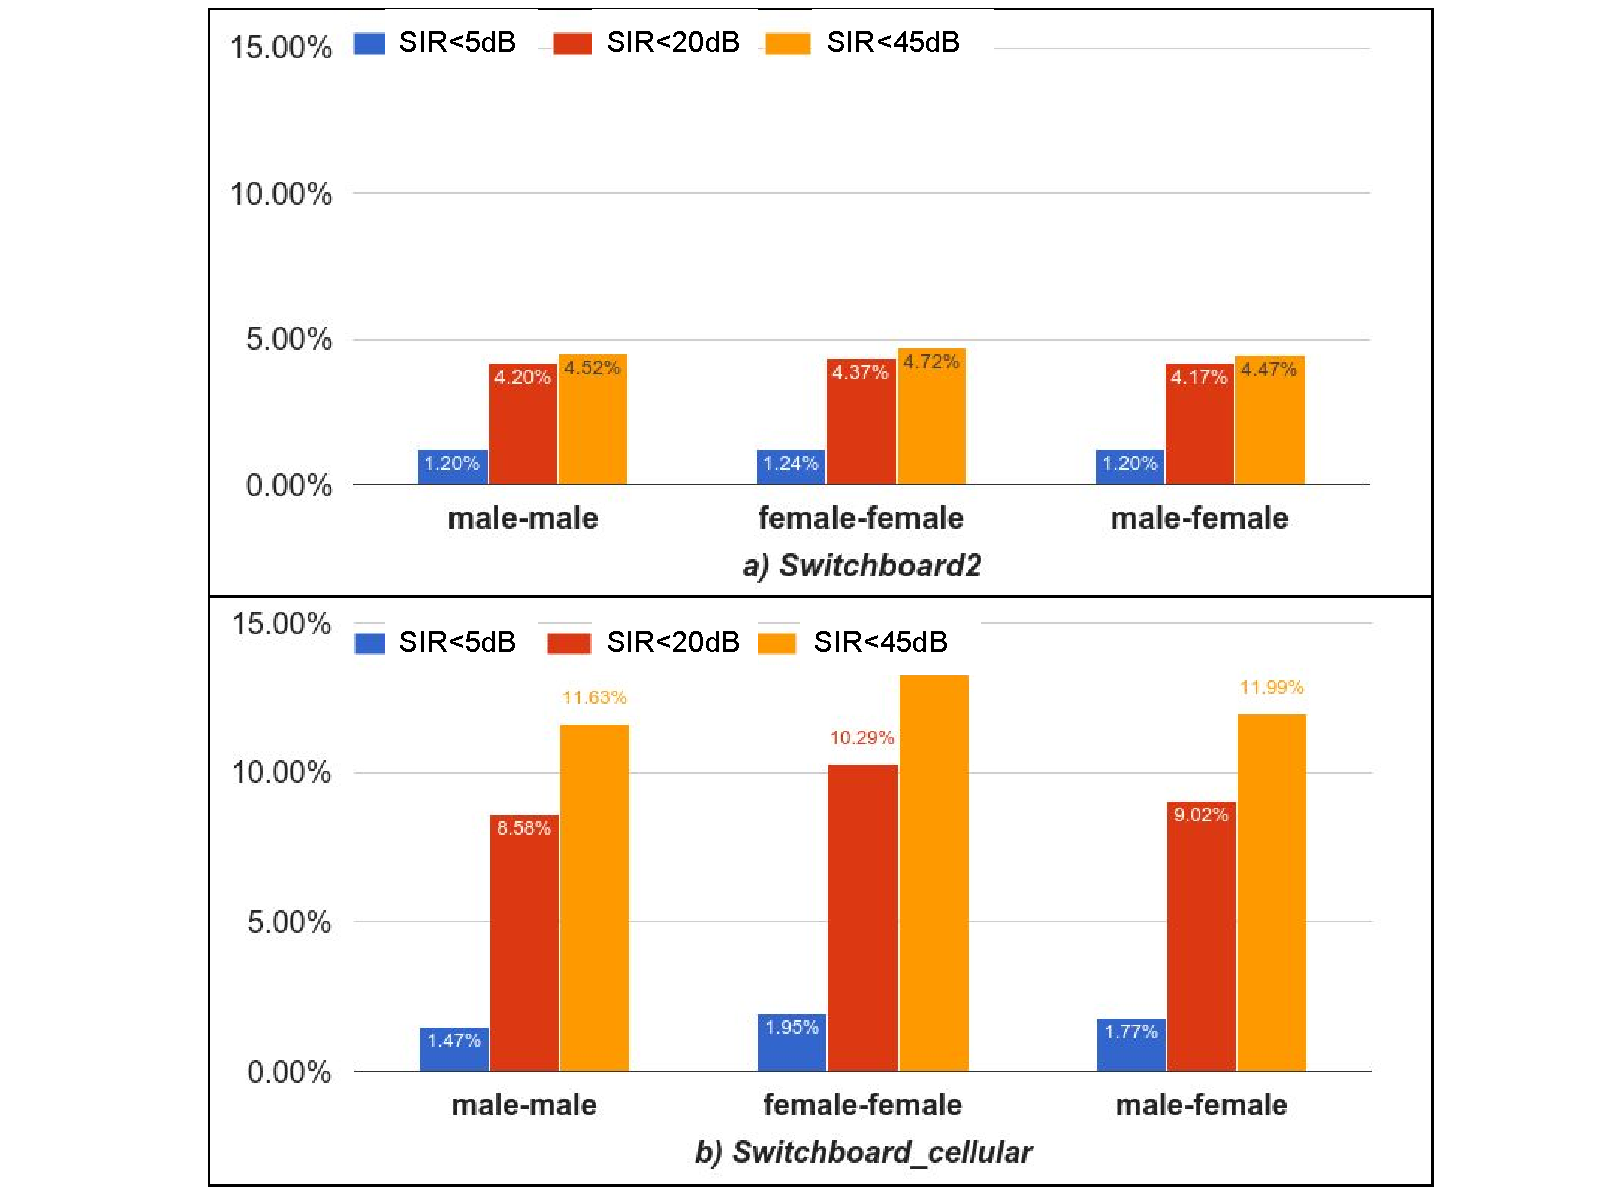
\includegraphics[height = 4in, width=0.8\textwidth]{figures/swb_overlap_percentage-crop}
	\vspace{-1mm}
	\caption{\it \small Percentage of overlaps to total speech in Switchboard2 and Switchboard cellular telephone conversations. Three SIR upper bounds are selected to label overlaps; 5dB, 20dB, 45dB. The higher the SIR upper bound, the stricter the overlap labels. Separate results are shown for male-male, male-female, and female-female conversations.}
	\label{fig:swb_overlap_percentage}
	\vspace{-3mm}
\end{figure*}


\begin{figure}[b!]
	\vspace{0mm}
	\centering
	\textbf{Overlap in meetings}\par\medskip
	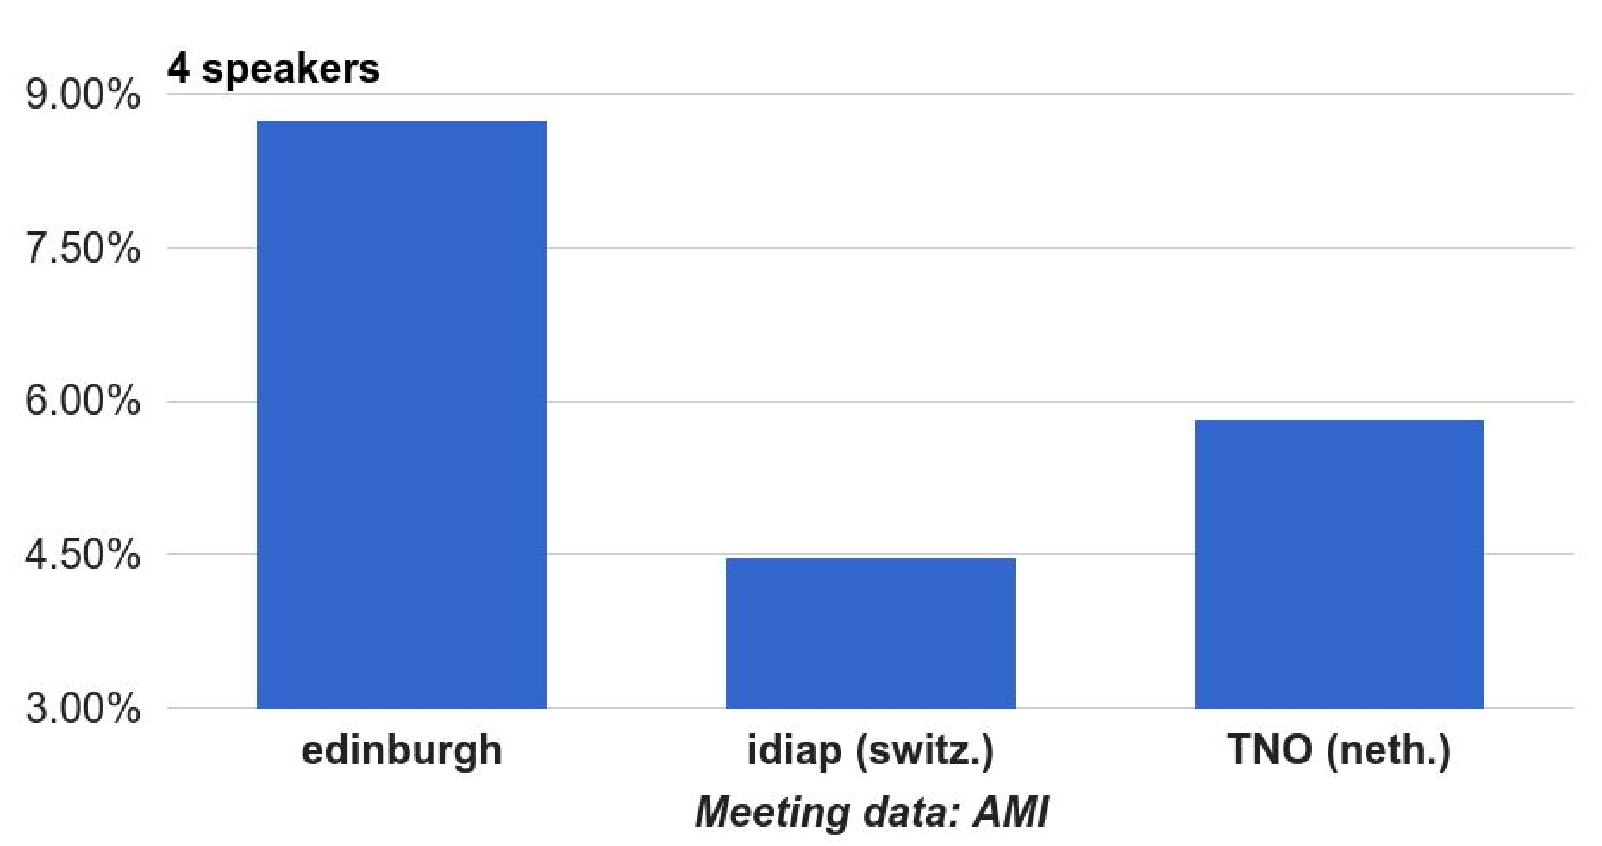
\includegraphics[height = 2.8in, width=0.5\textwidth]{figures/ami_overlap_percentage-crop}
	\vspace{-3mm}
	\caption{\it \small Percentage of overlaps to total speech in the AMI meeting corpus. All meetings used here have exactly 4 speakers. 
	The percentage of overlap is significantly higher here compared to Switchboard (compare with blue bars in Fig.~\ref{fig:swb_overlap_percentage}).}
	\label{fig:ami_overlap_percentage}
	\vspace{-3mm}
\end{figure}


To investigate the amount of overlap in conversational speech, two popular corpora are examined here: 
\begin{itemize}
	\item Switchboard2: a large collection of five minute telephone conversations involving several hundred speaker from across the United States.
	\item Switchboard Cellular: five-six minute telephone conversations on cellular phones.
	\item AMI meeting corpus: A dataset consisting of 100 hours of meeting recordings from several locations across Europe. 
\end{itemize}
For each session, the separate (almost interference-free) channels provided for each speaker are first segmented into speech and silence using an energy-based speech activity detection. 
Signal energies are required for each time-frame ($25msec window$), since signal-to-interference ratio (SIR) is used to define overlap. 

\begin{equation}
\label{eq:abs_sir}
SIR(n) = 10log_{10}(\frac{P_1(n)}{P_2(n)})
\end{equation}
where $P_1(n)$ is the per-frame energy of channel 1 and $P_2(n)$ corresponds to channel 2. $n$ represents frame indexes. 
Channels are mixed (per sample addition of the two signals) to create co-channel data. 
Instances at which both speakers are active are considered overlapped. 
Since the SIR value varies for different segments, we use a threshold on the SIR to label frames as overlapped. 
Segments with absolute SIR (i.e., $|SIR|$) lower than the threshold are considered overlapped.
The amount of overlap varies with the maximum allowable SIR (i.e., threshold) set by the evaluator. 
For instance, one might consider the mere presence of two speakers at the same time sufficient to label a segment as overlap, which is an indication of high SIR thresholds ($45dB$ in Fig.~\ref{fig:swb_overlap_percentage}). 
A more pragmatic view, however, is to choose an SIR small enough to preserve as much data possible. 
This way of preserving some overlapped segments is shared in many studies under the definition of usable speech~\cite{yantorno_report,smolenski_tut}. 
Lower SIR values, $(0-5) dB$, have a more significant impact on speaker verification, but to provide more insight, three SIR upper bounds have been used in Fig.~\ref{fig:swb_overlap_percentage}; $5$, $20$, $45dB$. 
We argue that any overlap up to $5dB$ should have noticeable impact on speaker verification. 
An upper bound of $45dB$ is also chosen, since the percentage of overlap is constant beyond $45dB$. 
It is shown in Fig.~\ref{fig:swb_overlap_percentage} that with a $5dB$ threshold, the percentage of overlap to total speech is below $2\%$. 
For the curios reader, we have provided overlap percentages for three groups of conversations: male-male, male-female, and female-female pairs. 
It is clear that for Switchboard gender does not play a role in dictating overlap percentage. 

For a broader perspective, we also analyze the AMI meeting corpus. 
The difference between meetings and phone conversations is in the number of speakers and face-to-face interaction. 
we speculate that number of speakers increases overlap while on the other hand the fact that all speakers are present in the same room (i.e., face-to-face interaction) limits the amount of overlap. 
Another difference is that SIR is not as well defined for meetings as it is for two-party phone-calls, since multiple parties may be active at the same time. 
In Fig.~\ref{fig:ami_overlap_percentage}, we assume at least two speakers should have a relative SIR of up to $5dB$. 
Any additional speaker is evaluated with respect to the primary speaker, but with a $20dB$ threshold. 
As Fig.~\ref{fig:ami_overlap_percentage} suggests, location also plays a significant role in overlap percentage. 
The authors refrain from speculating the impact of location, since it exceed the scope of this study. 

In text-independent speaker recognition, where we are interested in long-term acoustic characteristics, 4-5\% of overlapped speech in our data has little effect on speaker recognition accuracy. 
The point here is not to say that overlapped speech can be neglected in speaker recognition, but to clarify that speaker recognition in its most common form is more concerned with co-channel speech in general rather than {\it overlap} as it appears in everyday English conversations. 
In the more general case of co-channel speech interference, the presence of secondary speakers has a significant impact on speaker verification. 
We roughly estimate that in a two-party phone conversation, approximately $50\%$ of the data contains the unwanted secondary speaker (compare this with $2\%$ in Fig.~\ref{fig:swb_overlap_percentage}). 
Section~\ref{ssec:cch_in_trials} will investigate the effect of overlap and co-channel on speaker verification EER. 



\subsection{Co-channel Interference in Trials}
\label{ssec:cch_in_trials}
In this section, a series of speaker verification experiments are conducted on Switchboard2 to demonstrate the effect of using co-channel speech in enrollment and test data. 
We do not introduce these experiments as ``baseline'', since it is an unfair assessment to add co-channel interference to trials and expect PLDA to perform well. 
The purpose of this section is to show the increase in equal error rates as a result of co-channel speech. 
We also further emphasize the point made in Sect.~\ref{sec:cochannl_in_sid} by identifying the impact of overlap from co-channel interference on the EER. 

\begin{figure*}[t!]
	\vspace{-1mm}
	\centering
	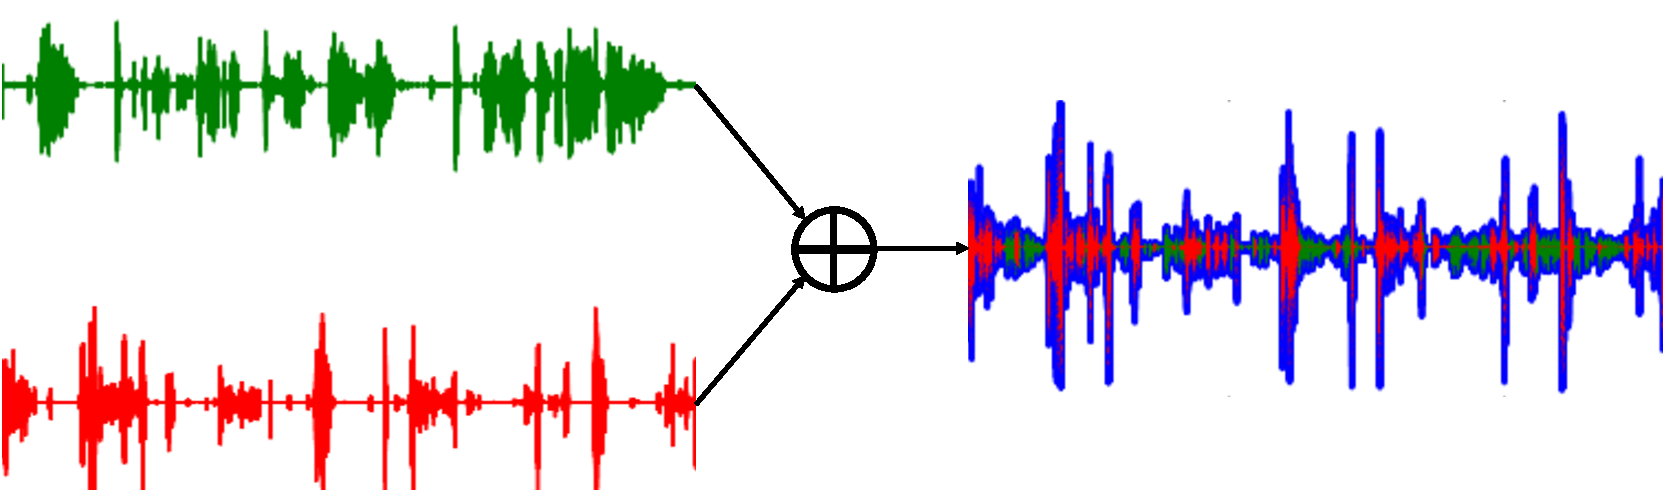
\includegraphics[height = 1.0in, width=0.45\textwidth]{figures/swb_cch_demo-crop}
	\vspace{-1mm}
	\caption{\it \small Mixing two channels of a Switchboard phonecall. The example here mixes the signals with 0dB SIR. Blue shows the resulting co-channel signal. Red and green each show one of the single-speaker signals.}
	\label{fig:mix_swb}
	\vspace{-1mm}
\end{figure*}

For these experiments, single-speaker data is used to estimate PLDA parameters (not co-channel data). 
Trials are evaluated at different levels of co-channel interference (i.e., SIR level). 
In each scenario, trial recordings are summed with their counterpart channel from the phone conversation to create co-channel data, as if speakers are speaking on a single channel (shown in Fig.~\ref{fig:mix_swb}). 
Speaker labels for trial recordings are generated based on the foreground speaker. 
In this context, foreground speaker refers to the speaker of interest. 
For example, in a $5dB$ co-channel session generated from Switchboard2 containing speakers {\bf X} and {\bf Y}, if {\bf X} were the foreground speaker, the average energy of {\bf X} would be $5dB$ higher than the average energy of {\bf Y}. 
%Therefore, $SIR_{trial}$ is defined slightly differently from here on after, compared to the per-sample absolute $SIR(n)$ in (\ref{eq:abs_sir}). 
%\begin{equation} 
%SIR_{trial} = 10log_{10}\Big(\frac{\frac{1}{T}\sum_t E_X(t)}{\frac{1}{T}\sum_t E_Y(t)}\Big), \hspace{30pt} t=1,...,N
%\end{equation}
%where $E_X(t)$ and $E_Y(t)$ are signal energies at frame $t$. 
Five SIR levels are chosen throughout experiments; $100dB$ (i.e., clean sessions), $20dB$, $10dB$, $5dB$, and $0dB$. 
In $0dB$ the average energy of the foreground and background data is equal. 
To avoid mismatch, the clean condition is also generated through the same procedure with an SIR of $100dB$ favoring the foreground speaker. 

A gender-independent universal background model (UBM) is created using 8kHz single-speaker NIST SRE data from 2004, 2005, and 2006 challenges~\cite{NIST04,NIST05,NIST06}. 
The UBM consists of $2048$ Gaussian mixtures representing a 39 dimensional feature space (13 dimensional MFCC plus $\Delta$ and $\Delta\Delta$). 
The same data from SRE 2004-6 is used to estimate a total variability (TV) matrix, which extracts $400$ dimensional i-vectors~\cite{Dehak_ivector}. 
The data used here to estimate PLDA parameters are single-speaker recordings from NIST SRE 2008~\cite{NIST08}. 
PLDA training data consists of approximately $11k$ single-speaker utterances from over $1300$ speakers. 
Trial data is developed from 2500 Switchboard2 recording sessions containing approximately $800$ speakers. 
Prior to feature extraction, trials are processed using comboSAD, an unsupervised speech activity detection~\cite{sadjadi2013unsupervised}. ComboSAD has previously shown to provide stable performance improvement in such speaker recognition tasks~\cite{hasan2013crss}. 

Figure~\ref{fig:cch_in_sid} shows speaker verification performance for the five SIR cases. 
As shown, EER for the clean condition is significantly lower than all the other SIR levels, even $20dB$. 
The sudden jump in EER shows the significance of co-channel interference. 

\begin{figure}[h!]
	\centering
	\textbf{Speaker recognition in co-channel}\par\medskip
	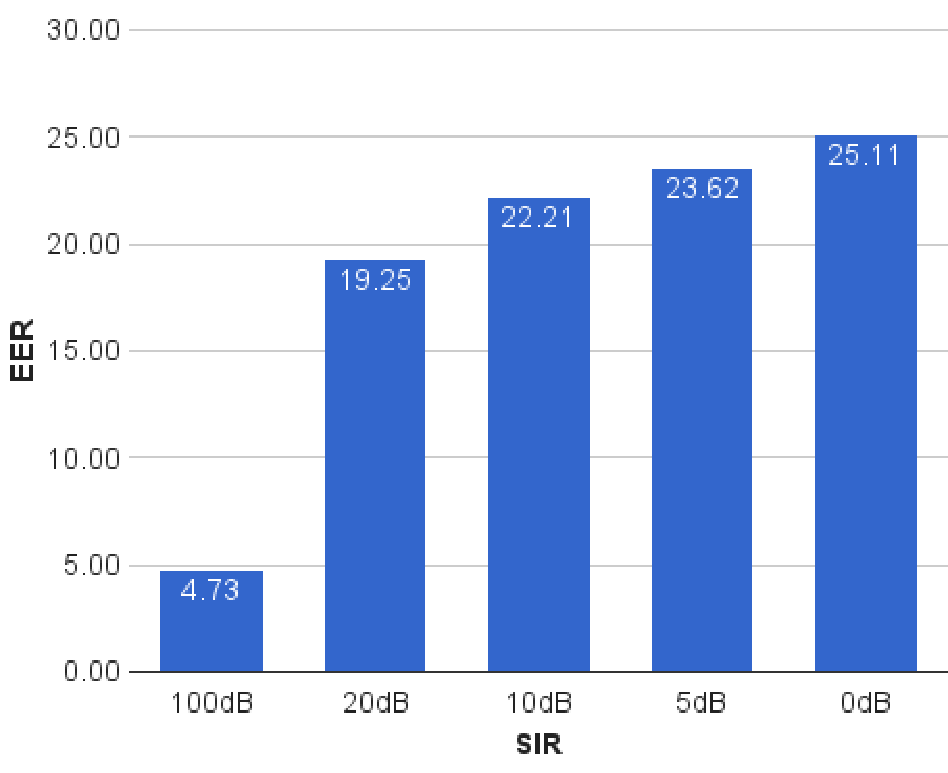
\includegraphics[height = 2.8in, width=0.5\textwidth]{figures/eer_vs_sir_swb2_baseline}
	\vspace{-2mm}
	\caption{\it \small Speaker verification performance with co-channel speech in switchboard trials. The i-vector/PLDA system uses a typical system configuration and is fully trained on single-speaker data. The purpose of this chart is to show the rapid increase in equal error rate (EER) as co-channel data is added to the trials. 100dB SIR represents clean (single-speaker) trials.}
	\label{fig:cch_in_sid}
	\vspace{-1mm}
\end{figure}

A second experiment is conducted to separate performance drop caused by overlap. To show this, all speech from the secondary speaker is dropped from the recordings, except for segments that overlap with the foreground speaker. 
This is accomplished by using voice activity detection (VAD) labels from the 100dB trials, while using $0dB$ audio data for the trials. 
Figure~\ref{fig:ovl_in_sid}, compares speaker verification under overlap with 0dB co-channel speech. 

\begin{figure}[h!]
	\vspace{-1mm}
	\centering
	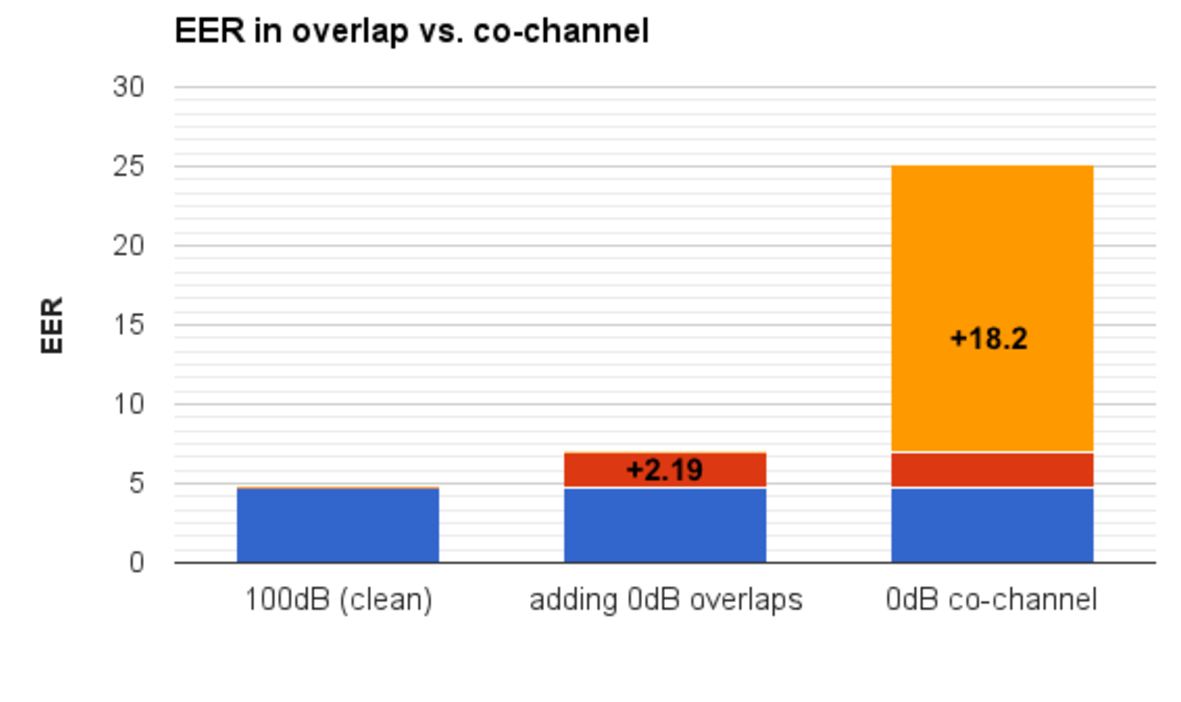
\includegraphics[height = 2.8in, width=0.5\textwidth]{figures/overlap_vs_cochannel_sid-crop}
	\vspace{-8mm}
	\caption{\it \small Comparing the effect of overlap in speaker verification with the more general case of co-channel. This study differentiates overlap from co-channel speech by considering overlaps to be segments during which both speakers are active. Co-channel refers to the more general case of two speakers in an audio stream, not necessarily overlapped (see Fig.~\ref{fig:cochannel_vs_overlap}). The chart shows that overlap plays a small part in the rise of EER compared to co-channel interference.}
	\label{fig:ovl_in_sid}
	\vspace{-1mm}
\end{figure}


\section{Motivation}
\label{sec:background}
Before presenting our proposed methods, it is essential to provide a brief overview of the chronological introduction and development of probabilistic linear discriminant analysis (PLDA) in speaker recognition. 
PLDA was initially proposed for face recognition in~\cite{prince_plda}. 
It was later adopted as a channel compensation step for speaker recognition using i-vectors~\cite{kenny2010bayesian}. 
A number of studies since then have presented different formulations for the factor loading paradigm most commonly known as PLDA. 
In this study, we are specifically interested in three formulations: 1) standard PLDA~\cite{kenny_plda}, 2) simplified PLDA~\cite{kenny_plda2,Daniel2011is}, and 3) the two-covariance model~\cite{brummer2010twocov}. 
The nomenclature used here is adopted from a recent study by Sizov et al.~\cite{sizov2014unifying} aimed at unifying the variations proposed for PLDA over the past decade. 


\subsection{Standard PLDA}
\label{ssec:standard_plda}
The general idea of probabilistic linear discriminant analysis is to find a subspace in the i-vector space that best represents speaker-specific components. 
The search for this subspace is based on a training dataset organized in a way that emphasizes differences between speakers as well as variations of each speaker across different recordings (aka sessions). 
The data organization comprises $n_i$ observation i-vectors for speaker $i$ from a set of development speakers, PLDA assumes the following linear factorization for each i-vector ${\bf m}_{ij}$: 

\begin{equation}
\label{eq:std_plda}
{\bf m}_{ij} = {\bf m}_g + {\bf V}{\bf y}_i+{\bf U}{\bf x}_{ij}+{\bf z}_{ij},  \hspace{30pt} j=1,...,n_i
\end{equation}
where $m_g$ represents the global i-vector mean. Speaker- and session-dependent latent variables, ${\bf y}_i$ and ${\bf x}_{ij}$, take a standard normal distribution, $\mathcal{N}({\bf 0},{\bf I})$. ${\bf V}$ and ${\bf U}$ are typically tall matrices representing eigenvoice and eigenchannel subspaces, respectively. Eigenvoice refers to the collection of factor loadings (represented in ${\bf V}$) that construct the speaker-dependent subspace. Eigenchannel refers to the session-dependent subspace. 
In addition to the eigenchannel subspace a session-dependent and normally distributed slack variable, ${\bf z}_{ij}$, is included to express session variabilities. In (\ref{eq:std_plda}), $z_{ij}$ takes a diagonal covariance matrix, $\mathcal{N}({\bf 0},{\bf \Sigma_d})$,~\cite{kenny_plda,prince_plda}. 
PLDA predicts model parameters, $({\bf V},{\bf U},{\bf \Sigma_d})$, using the expectation-maximization (EM) algorithm~\cite{prince_plda}. 
After estimating subscpace components using background development data, trial i-vectors are reduced to the same speaker-dependent subspace using PLDA and scored through a hypothesis testing procedure (see~\cite{prince_plda} for details). 
The hypothesis testing stage estimates the likelihood ratio of whether two trial i-vectors (train and test) belong to the same speaker, or if they belong to two different speakers. 

\subsection{Simplified PLDA}
\label{ssec:simplified_plda}
The second formulation reduces complexity in (\ref{eq:std_plda}) using the fact that session-dependent latent variables (${\bf x}_{ij}$ in (\ref{eq:std_plda})) are not directly used in the scoring process. 
Therefore, as long as models are able to effectively estimate the eigenvoice subspace, channel-dependent components (essentially all non-speaker dimensionality) are redundant. 
With this in mind, the second term in (\ref{eq:std_plda}) is removed in simplified PLDA and all channel information is captured in the slack variable. 
The slack variable in this case is assumed to have a full covariance matrix.

\begin{equation}
\label{eq:simple_plda}
{\bf m}_{ij} = {\bf m}_g + {\bf V}{\bf y}_i+{\bf z}^f_{ij}.  \hspace{30pt} j=1,...,n_i
\end{equation}
The use of a full covariance matrix in the slack variable can be interpreted as combining the diagonal slack covariance in (\ref{eq:std_plda}) with the eigenchannel subspace projection ${\bf UU}^T$~\cite{sizov2014unifying}.
We consider this formulation our baseline. 

\subsection{PLDA as an extension to LDA}
\label{sec:twocov}
The last interpretation, called the two-covariance model~\cite{sizov2014unifying}, is a probabilistic extension to linear discriminant analysis (LDA). 
The two-covariance model describes the i-vector space in terms of between- and within-speaker covariances, as does LDA. 
It is well known that LDA models feature spaces as a mixture of Gaussians, in which each mixture has the same covariance, ${\bf \Phi_w}$. 
Gaussian mixtures represent within-class (i.e., session) variability, therefore ${\bf \Phi_w}$ is referred to as the within-class covariance matrix. 
LDA is commonly used to find the optimal discriminating subspace of a given set of training speakers, relative to their within-speaker variation~\cite{ioffePLDA2006}. 
The problem, however, is that the aforementioned subspace is only optimal for the given training speakers. 
What LDA fails to provide is a continuous (or in this context, stochastic) representation of each mixture's centroid\footnote{In i-vectors, centroids are known to correspond to speakers. In other words, each centroid represents a speaker.}. 
Therefore, centroids are considered deterministic in LDA. 
When a new speaker is introduced, the resulting projection of LDA is not necessarily reliable. 
PLDA provides a stochastic representation of class centroids using a between-class covariance matrix, ${\bf \Phi_b}$~\cite{ioffePLDA2006}. 
The centroid distribution assumes a continuous centroid subspace, which acknowledges the possibility of unseen speakers. 
PLDA can therefore be defined as a combination of two distributions; 
\begin{enumerate}
	\item the distribution of i-vectors in each class representing a certain speaker, which is a Gaussian with mean $m_c$, mean of a speaker's i-vectors, and covariance ${\bf \Phi_w}$. $c$ here represents the class label, or speaker identity. Therefore, the probability of an i-vector, $m$, given that it comes from class $c$ is:
	\begin{equation}
	\label{eq:within_spk_dist}
	{\bf m} \sim \mathcal{N} ({\bf m}_c,{\bf \Phi_w} | c),
	\end{equation}
	\item the class centroid distribution, also assumed Gaussian:
	\begin{equation}
	\label{eq:between_spk_dist}
	{\bf m}_c \sim \mathcal{N} ({\bf m}_g,{\bf \Phi_b}),
	\end{equation}
	where ${\bf m}_g$ is the global mean of all class centroids (assumed to be equal to the global mean of all i-vectors) and ${\bf \Phi_b}$ is the between-speaker covariance matrix. 
\end{enumerate}

Defining channel variability as a function of speaker variation helps PLDA model unseen speakers (i.e., speakers that are not present in the development set). 
As opposed to LDA, which is incapable of offering optimal solutions to speakers that are absent from the training set~\cite{ioffePLDA2006}. 
The interpretation in this section, provides a perspective which we will use in our proposed method (Sect.~\ref{sec:cch_plda}) to investigate adding co-channel interference as a contributor to within-class variability. 
Using a transformation matrix (${\bf V}$), equations (\ref{eq:within_spk_dist}) and (\ref{eq:between_spk_dist}) can be translated to (\ref{eq:simple_plda})~\cite{sizov2014unifying} in which the within- and between-covariances are diagonalized~\cite{ioffePLDA2006}. 


\section{Proposed method: mixed PLDA}
\label{ssec:plda_data_prep}
The search for eigenvoice and eigenchannel subspaces involves a careful selection of development data. 
The idea in data preparation for PLDA is to provide sufficient channel diversity for each speaker to model within-speaker variations, while maintaining high speaker counts to model between-speaker variability. 
Channel and speaker variation introduced in the development data are directly translated into within- and between-speaker covariances, respectively. Said covariances are used to estimate PLDA parameters, (\ref{eq:std_plda}) and (\ref{eq:simple_plda})~\cite{sizov2014unifying}. 
The data-driven perspective towards channel compensation using PLDA has inspired a number of studies to address other types of variability through the same data selection procedure, where instead of channel diversity, one could generate a development set with age~\cite{kelly2013} or language diversity~\cite{misra2014languagemismatch} (in the case of multi-lingual speakers). 
Therefore, our first approach is to investigate co-channel speaker recognition performance when background PLDA data contains co-channel speech recordings. 

Co-channel recordings for each speaker are obtained from separate conversations. In these conversations, it is important to maintain diversity in secondary (aka interfering) speakers; since without sufficient secondary speaker diversity, the PLDA model will train to both primary and secondary speakers. 
Figure~\ref{fig:mixedPLDA_diagram} is a diagram of how the PLDA data is arranged in this approach, which we call ``mixed PLDA''. 
Mixed PLDA introduces speaker interference in the background development data using co-channel mixtures to implicitly train the PLDA model to recognize speaker interference as session variability. 


\begin{figure}[t!]
	\centering
	\vspace{0mm}
	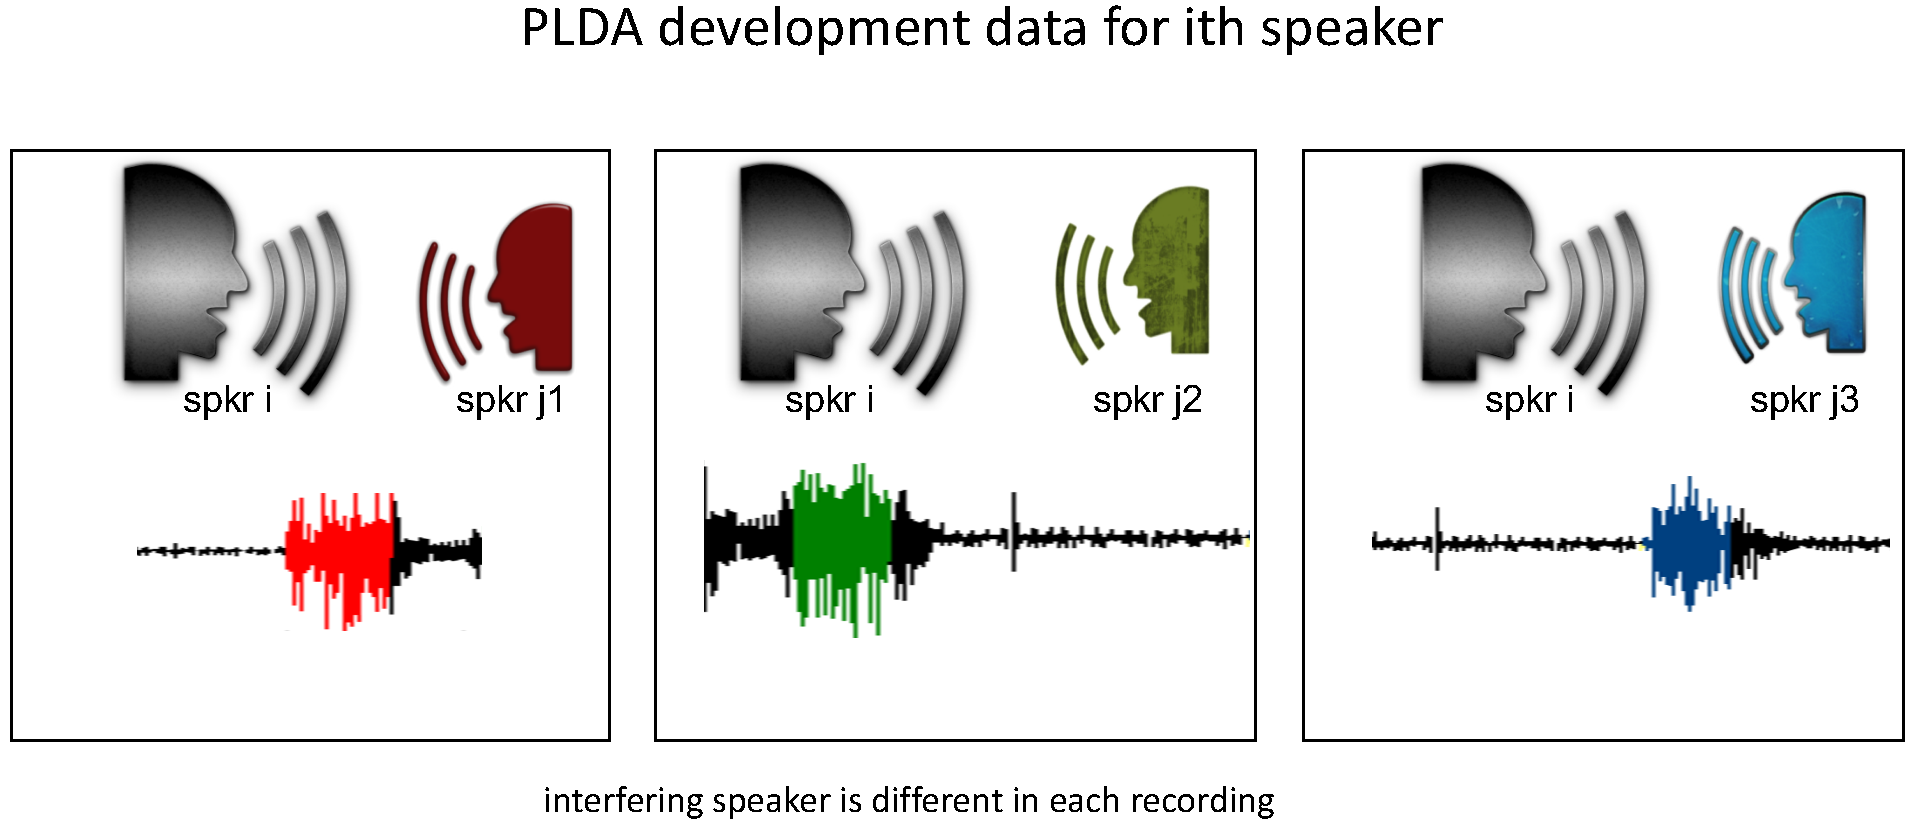
\includegraphics[width=0.6\textwidth, height=2in]{figures/mixedPLDA_slide-crop}
	\vspace{0mm}
	\caption{\it \small Creating development data for co-channel aware PLDA. the mixed PLDA approach uses co-channel data for each speaker in the background model. Recordings for the $i^{th}$ speaker consists of co-channel sessions with different speakers.}
	\label{fig:mixedPLDA_diagram}
	\vspace{-3mm}
\end{figure}

Mixed PLDA describes the use of co-channel background data in simplified PDLA, (\ref{eq:simple_plda}). 
This will be used as a baseline to provide fair comparison with our proposed PLDA formulation described in the next section. 

\subsection{Co-channel Interference in Trials with mixedPLDA} 
\label{sssec:mixedplda_exp}

Now that we have introduced {\it mixed PLDA}, we evaluate its performance by adding co-channel data to the PLDA training set. 
There are a number of ways co-channel data can be inserted, particularly in the choice of SIR. 
We investigate three cases in our experiments: 
\begin{itemize}
	\item $0dB$: All co-channel data used to train PLDA is 0dB. 
	\item $(0,100)dB$: Half of the data is clean and the other half is $0dB$. 
	\item $(0,5,10,20,100)$: co-channel files are uniformly selected from one of these five SIR values. 
\end{itemize}

Table~\ref{tbl:mixed_plda} shows that mixed PLDA with half $0dB$ and half $100dB$ co-channel training data for PLDA causes the least damage in the clean condition (a.k.a $100dB$), from $4.73$ to $5.22$. Mixed PLDA ($0$,$100dB$) also reduces error rates the most. 
Minimum detection cost functions (minDCF) is calculated over the operating point ($C_{fa}=10, C_{miss}=1, prior = 0.001$). 
These observation are consistent with those reported in~\cite{shokouhi2015probabilistic}. 

\begin{table*}[b!]
	\small
	\centering
	\resizebox{\textwidth}{!}
	{
		\begin{tabular}{|l|c|c|c|c|c|c|c|c|c|c|c|}
		\hline
		\multirow{2}{*}{SIR (dB)} & \multicolumn{3}{c|}{mixed PLDA (0dB)}          & \multicolumn{3}{c|}{mixed PLDA (0,5,10,20,100dB)}  & \multicolumn{3}{c|}{mixed PLDA (0,100dB)}       & \multicolumn{2}{l|}{simplified PLDA} \\ \cline{2-12} 
		& \multicolumn{2}{r|}{EER (\%)} & minDCF         & \multicolumn{2}{c|}{EER (\%)} & minDCF             & \multicolumn{2}{c|}{EER (\%)} & minDCF          & EER(\%)           & minDCF           \\ \hline
		100                       & \multicolumn{2}{c|}{7.48}     & 0.587          & \multicolumn{2}{c|}{5.71}     & 0.809              & \multicolumn{2}{c|}{\bf 5.22}     & 0.472           & 4.73              & 0.407            \\ \hline
		20                        & \multicolumn{2}{c|}{19.75}    & 0.897          & \multicolumn{2}{c|}{17.49}    & 0.865              & \multicolumn{2}{c|}{\bf 17.14}    & 0.872           & 19.25             & 0.909            \\ \hline
		10                        & \multicolumn{2}{c|}{21.79}    & 0.941          & \multicolumn{2}{c|}{20.24}    & 0.923              & \multicolumn{2}{c|}{\bf 19.82}    & 0.918           & 22.21             & 0.944            \\ \hline
		5                         & \multicolumn{2}{c|}{23.20}    & 0.960          & \multicolumn{2}{c|}{21.86}    & 0.948              & \multicolumn{2}{c|}{\bf 21.02}    & 0.940           & 23.62             & 0.967            \\ \hline
		0                         & \multicolumn{2}{c|}{24.61}    & 0.976          & \multicolumn{2}{c|}{23.13}    & 0.971              & \multicolumn{2}{c|}{\bf 22.43}    & 0.963           & 25.11             & 0.985            \\ \hline
	\end{tabular}
	}
	\caption{Mixed PLDA: PLDA performance when co-channel interference is introduced as session variation, without changing the original PLDA formulation. The EER for simplified PLDA is presented in the last column for comparison. }
	\label{tbl:mixed_plda}
\end{table*}

It is interesting that the best performance is obtained with a 50-50 split of co-channel and clean data in the PLDA training set. 
At this point I do not have a clear explanation of why {\it mixed PLDA} ($0,100dB$) is superior to ($0dB$) or ($0,5,10,20,100dB$). 

\section{Proposed method: dual eigenvoice PLDA}
\label{sec:dualev_plda}

The approach in {\it mixed PLDA} relies on the ability of PLDA that compensates channel mismatch. 
PLDA recognizes the variabilities observed across different recordings for a given speaker and removes them from the speaker subspace (aka the eigenvoice factors in ${\bf V}$). 
Therefore, {\it mixed PLDA} treats interfering speech as channel mismatch. 
This is accomplished by adding co-channel i-vectors to the PLDA background data and leaving it to the PLDA model estimation process to recognize interfering speech and remove its effects in the speaker subspace. 
However, interfering speech is not effectively picked up by neither the eigenchannel matrix (in case of the standard PLDA in~(\ref{eq:std_plda})) nor the slack variable, in (\ref{eq:simple_plda}). 
We address this by introducing our second approach which is to add a speaker dependent term intended to model interfering speech. Since the second term also corresponds to speaker identities, it should as well be represented by the speaker subspace. 
We call this approach {\it dual eigenvoice PLDA}, for which the PLDA factorization is: 

\begin{equation}
\label{eq:cchplda}
{\bf m}_{ij} = {\bf V}{\bf y}_i+{\bf V}^\prime {\bf w}_{ij}+{\bf z}_{ij}.
\end{equation}
Since the model still needs to represent channel variabilities, we keep ${\bf z}_{ij}$ as a full covariance normal distributed vector. 
${\bf V}^\prime$ represents the speaker dependent subspace, as does ${\bf V}$, with the difference that one is a rotation of the other with an unknown rotation factor. 
${\bf w}_{ij}$ is the latent variable which corresponds to the interfering speaker. 
There are a few reasons that prevent us from directly using ${\bf V}$ as factor loadings for the interfering components in~(\ref{eq:cchplda}), one being that as part of the degrees of freedom in the PLDA solution, the eigenvoice matrix can only be determined up to an unknown rotation matrix~\cite{sizov2014unifying} (similarly for ${\bf V}^\prime$). 
Equation (\ref{eq:cchplda}) uses different notation for the second eigenvoice matrix to remind us of this limitation. 
This prevents directly using ${\bf V}$ to represent the interfering speaker term. However, since we know that ${\bf V}$ and ${\bf V}^\prime$ must be related by a rotation matrix, we can use this knowledge to simultaneously update ${\bf V}$ and ${\bf V}^\prime$ in the EM iterations. 

As discussed, the relation between ${\bf V}$ and ${\bf V}^\prime$ is characterized by an unknown rotation matrix, ${\bf R}$:

\begin{equation}
{\bf V} = {\bf RV}^\prime.
\end{equation}
A reasonable ${\bf R}$ can be estimated via singular value decomposition (SVD) by considering the columns of ${\bf V}$ and ${\bf V}^\prime$ as data points in the speaker dependent subspace. The rotation matrix is derived from the cross-variance between ${\bf V}$ and ${\bf V}^\prime$ basis functions, ${\bf S}$:

\begin{equation}
{\bf S} = {\sum\limits_{i=1}^{N_V}\tilde{{v}_i}\tilde{{v}^\prime_i}^T},
\end{equation}
where $\tilde{v_i}$ is $v_i$ are the eigenvoice basis vectors centered at the origin and $N_V$ is the number of columns in ${\bf V}$ (and/or ${\bf V}^\prime$, since both have the same dimensions). The rotation matrix is defined as below:

\begin{equation}
{\bf R} = {\bf S}_{row}{\bf S}_{col}^T,
\end{equation}
where $S_{col}$ and $S_{row}$ are the column and row spaces of ${\bf S}$ obtained from SVD:

\begin{equation}
{\bf S} = {\bf S}_{col}{\bf \Lambda}{\bf S}_{row}^T.
\end{equation}

The rotation matrix is used in each iteration of the EM algorithm to update the matrix ${\bf V}^\prime$ and align it with ${\bf V}$, 

\begin{equation}
{\bf V}^\prime \leftarrow {\bf RV^\prime}. 
\end{equation}

Updating ${\bf V}^\prime$ before estimating the statistical statistics of latent variables, $y_{i}$ and $w_{ij}$, removes the redundancy in the second term of equation~(\ref{eq:cchplda}) by replacing the eigenvoice matrix ${\bf V}^\prime$ with information obtained from the basis vectors in ${\bf V}$. Since both factors in~(\ref{eq:cchplda}) are guided towards representing the speaker space, the overall system achieves a better estimate of ${\bf V}$ and Consequently more accurate estimates for latent variable statistics. 

\subsection{Co-channel Interference in Trials with dual eigenvoice PLDA} 
\label{ssec:dualevplda_exp}

\begin{figure*}[b!]
	\centering
	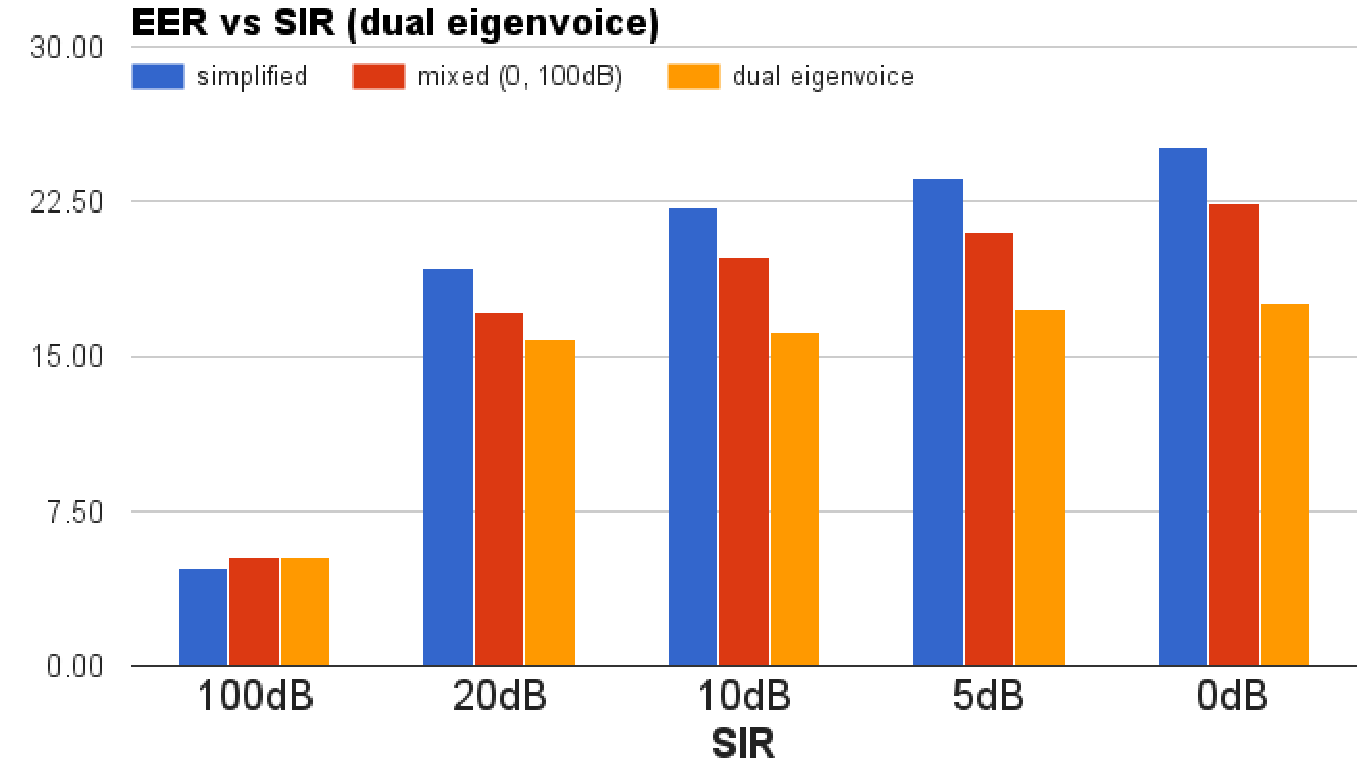
\includegraphics[height = 2.5in, width=0.5\textwidth]{figures/eer_vs_sir_dualeigenvoice}
	\vspace{-2mm}
	\caption{\it \small Comparing {\it dual eigenvoice PLDA}(yellow) with {\it mixed PLDA} (red) and {\it simplified PLDA} (blue). A steady improvement over {\it mixed PLDA} is observed across co-channel conditions. }
	\label{fig:eer_dualeigenvoice}
	\vspace{-1mm}
\end{figure*}

As described in Sect.~\ref{sec:dualev_plda}, {\it dual eigenvoice PLDA} attempts to model a linear factorization of the i-vectors into a target speaker and an interfering speaker component (see Eq.~(\ref{eq:cchplda})). 
PLDA is able to distinguish the target speaker using the several recordings available for each speaker. 
The key difference between this method and {\it mixed PLDA} is that the system is forced to use a similar subspace to model the interfering speaker. 
Figure~\ref{fig:swb_sid_results} shows the EER for different amounts of co-channel interference introduced to the trials. 

Considering that {\it simplified PLDA} does not claim robustness towards co-channel interference, it shows little resistance as trial SIR values increase. 
Since {\it mixed PLDA} has some observation of the co-channel condition, it reduces the EER for at least 1\% across all SIR conditions, as was shown in Sect.~\ref{sssec:mixedplda_exp}. {\it Dual eigenvoice PLDA}, further improves the performance and obtains 2.5-3.5\% drop in EER in all conditions. EER variations are significantly different for {\it dual eigenvoice PLDA} model compared to the other two systems. 
Figure~\ref{fig:eer_dualeigenvoice} shows that the clean-to-$0dB$ EER range for {\it mixed PLDA} is more than twice as much as {\it dual eigenvoice PLDA}. 



\subsection{convergence of Dual eigenvoice PLDA}
\label{ssec:convergence_dualevplda}
An interesting observation was made while developing {\it dual eigenvoice PLDA} regarding the convergence of model parameters, specifically the second eigenvoice matrix. 
Later, with some more investigation and feedback from experts in the field, I realized a significant flaw in the proposed formulation. 
This section provides a brief description of the issue with {\it dual eigenvoice PLDA}. 

The claim in {\it dual eigenvoice PLDA} is that the first eigenvoice matrix in (\ref{eq:simple_plda}) contains factor loadings corresponding to the primary speaker and the second eigenvoice matrix (i.e., ${\bf V}^\prime$) is for secondary speakers. 
We also chose a full-covariance slack variable, ${\bf z}$. 
The problem here arises from the full-covariance slack variable. 


\section{Proposed method: Co-channel Aware PLDA}
\label{sec:cch_plda}
This section describes our proposed approaches, which are modifications to the PLDA formulation (Sect.~\ref{sec:background}) that allow modeling speaker interference in ways that are more appropriate for co-channel speech. 
Previously, in~\cite{shokouhi2015probabilistic}, we proposed a modified PLDA formulation to remove secondary speaker interference from the latent variable subspace. 
This study uses different methods based on the two-covariance interpretation (described in Sect.~\ref{sec:twocov}). 
%Part of the reason for our departure from the co-channel PLDA formulation proposed in~\cite{shokouhi2015probabilistic} was our inability to justify certain behavior in the model. 
Our method, which we call {\it co-channel aware PLDA} (caPLDA), uses the dual distribution definition of (\ref{eq:within_spk_dist}) and (\ref{eq:between_spk_dist}) to model a co-channel i-vector. 

As mentioned before, caPLDA adopts the two-covariance interpretation of PLDA briefly described in (\ref{eq:within_spk_dist}) and (\ref{eq:between_spk_dist}). 
The i-vectors of a given class can be modeled as a normally distributed vector with a mean pertaining to the class to which it belongs and a covariance matrix representing within class variability, (\ref{eq:within_spk_dist}). 
Typically, within-class variability is meant to model channel variation across sessions. 
In the case of co-channel speech, in addition to channel variability, one must consider the variability caused by interfering speakers. 
We will see in Sect.~\ref{ssec:cch_in_trials} that speaker interference has a dramatic impact on error rates. Much more compared to channel variation in a dataset such as Switchboard. 
It is therefore reasonable to prioritize co-channel interference over channel mismatch. 

In Sect.~\ref{ssec:plda_data_prep}, we proposed capturing speaker interference in the same manner that channel variation is captured by PLDA. 
Although some improvement is attainable, we expect that the original PLDA formulation, (\ref{eq:simple_plda}), is not capable of fully capturing speaker interference; partly due to the similarity between speaker-dependent latent variables and the cross-session variations that exist in co-channel interference. 

We propose that in order to improve performance, information can be shared from the between-speaker covariance to within-class covariances. 
For an i-vector with speaker $A$ as the foreground speaker and some speaker $X$ as secondary speaker, PLDA assumes a normal distribution $\mathcal{N} ({\bf m}_A,{\bf \Phi} | A)$. 
While (\ref{eq:within_spk_dist}), considers ${\bf \Phi}$ to be a unique within-class covariance matrix for all speakers in the i-vector space (i.e., $\Phi_w$), we argue that an additional component is required to model within speaker variations in the case of co-channel i-vectors. 
The additional component contributing to within-class covariance is of the same nature of the between-class covariance. 
Therefore, one can assume that ${\bf \Phi}$ is a function of both ${\bf \Phi}_w$ and ${\bf \Phi}_b$, $ \mathcal{F} ({\bf \Phi}_w,{\bf \Phi}_b)$. 
Our suggested structure for $ \mathcal{F} (.,.)$ is a linear combination of the two covariance matrices: 

\begin{equation}
\label{eq:complex_phiw}
\Phi = \mathcal{F} (\Phi_w,\Phi_b) = 
\alpha_w\Phi_w + \alpha_b\Phi_b
\end{equation}
where $\alpha_w$ and $\alpha_b$ are functions of the signal-to-interference ratio between the foreground and background speaker. 

We will visit different possibilities of $(\alpha_w, \alpha_b)$ in Sect.~\ref{sec:exp}. But first, we find it useful to focus on a special case, which is to assume session variability should be of the exact same type as speaker variability in the case of co-channel i-vectors. 
This special case assumes equal within- and between-speaker covariances. 

\subsection{Equal within- and between-speaker covariances ($\alpha_w = 0$)}
\label{ssec:alpha_w_0}
In~\cite{ioffePLDA2006}, PLDA model parameters are learned by maximizing the likelihood of observation i-vectors provided for each speaker (i.e., class). 
The likelihood is calculated by assuming the i-vectors are conditionally independent given the speaker. 
In this case, the probability of i-vectors $m^1, m^2, ..., m^n$ regardless of the speaker they were generated from, represented by $y$, is:

\begin{equation}
\mathcal{P}(m^1 m^2 ... m^n) = \int \mathcal{P}(y) \mathcal{P}(m^1 | y) \mathcal{P}(m^2 | y) ... \mathcal{P}(m^n | y) dy,
\end{equation}
Replacing the probabilities using (\ref{eq:within_spk_dist}) and (\ref{eq:between_spk_dist}), the log-likelihood of $\mathcal{P}(m^1 m^2 ... m^n)$ is: 


\begin{equation}
\label{eq:llk_twocov}
\begin{split}
\mathcal{L}(m^1 m^2 ... m^n) = -\frac{c}{2}(ln | {\bf \Phi}_b + \frac{1}{n}{\bf \Phi}_w | + tr(({\bf \Phi}_b + \frac{1}{n}{\bf \Phi}_w)^{-1}S_b) \\+ (n-1)ln|{\bf \Phi}_w| + ntr({\bf \Phi}_w^{-1}S_w)),
\end{split}
\end{equation}
where $S_b$ and $S_w$ are the between-speaker and within-speaker scatter matrices calculated from the training i-vectors. $c$ is a normalizing constant. 
The log-likelihood is maximized using (\ref{eq:llk_twocov}), resulting in expectation-maximization (EM) steps that estimate values for ${\bf \Phi}_w$ and ${\bf \Phi}_b$. 
If we ignore channel variability across sessions and assume that the only source of variation across different sessions is between-speaker variability, the probabilities $\mathcal{P} (x_i | y)$ change from $\mathcal{N} (y,\Phi_w)$ to: 

\begin{equation}
\mathcal{P} (x_i|y) = \mathcal{N} (y,\Phi_b).
\end{equation}

The assumption here is that within-session variation is similar to between-speaker variations (i.e., ${\bf \Phi}_b$). 
This assumption is equivalent to setting $\alpha_w$ to $0$ and $\alpha_b$ to $1$ in (\ref{eq:complex_phiw}). 
The upside of setting ${\bf \Phi}$ to ${\bf \Phi}_b$ is twofold: 1) it increases the accuracy of estimating ${\bf \Phi}_b$, since in this scenario within-speaker differences can also be used to calculate ${\bf \Phi}_b$. 2) The maximum likelihood problem in (\ref{eq:llk_twocov}) is reduced to:

\begin{equation}
\label{eq:llk_onecov}
\begin{split}
\mathcal{L}(m^1 m^2 ... m^n) = -\frac{c}{2}(nln | {\bf \Phi}_b | + ln(\frac{n+1}{n})+ \frac{n}{n+1}tr({\bf \Phi}_b^{-1}S_b) \\+ ntr({\bf \Phi}_b^{-1}S_b)),
\end{split}
\end{equation}
which is simpler to maximize. In fact, when all speakers have the same number of training i-vectors ($n$), the solution is to set $\Phi_b$ to $S_b$. 



\subsection{Co-channel Interference in Trials with caPLDA}
\label{ssec:caplda_exp}
Finally, we would like to analyze the potential gain in using alternative PLDA formulations described in Sect.~\ref{sec:cch_plda}. 
Instead of a grid-search of all possible $(\alpha_w,\alpha_b)$ inputs, only a selection of are presented here that we think provide most useful insight. 

Figure~\ref{fig:alpha_w_is_1}, shows the case in which $\alpha_w$ is set to $1$ and $alpha_b$ varies from $0$ to $1$. 
The EER values are almost unequivocally lower than their counterparts presented in Tab.~\ref{tbl:mixed_plda}, despite the fact that they do not use mixed PLDA training data. 
In other words, the EER values calculated in Fig.~\ref{fig:alpha_w_is_1} show performance using clean ($100dB$) PLDA training. 
The bottom line (blue) shows EER for clean trials. 
As expected, EER values slightly increase in the clean condition, when the original PLDA formulation is modified. 
However, in lower SIR conditions ($20-0dB$), more performance gain is observed as $alpha_b$ approaches $0.1$. 

\begin{figure*}[h!]
	\centering
	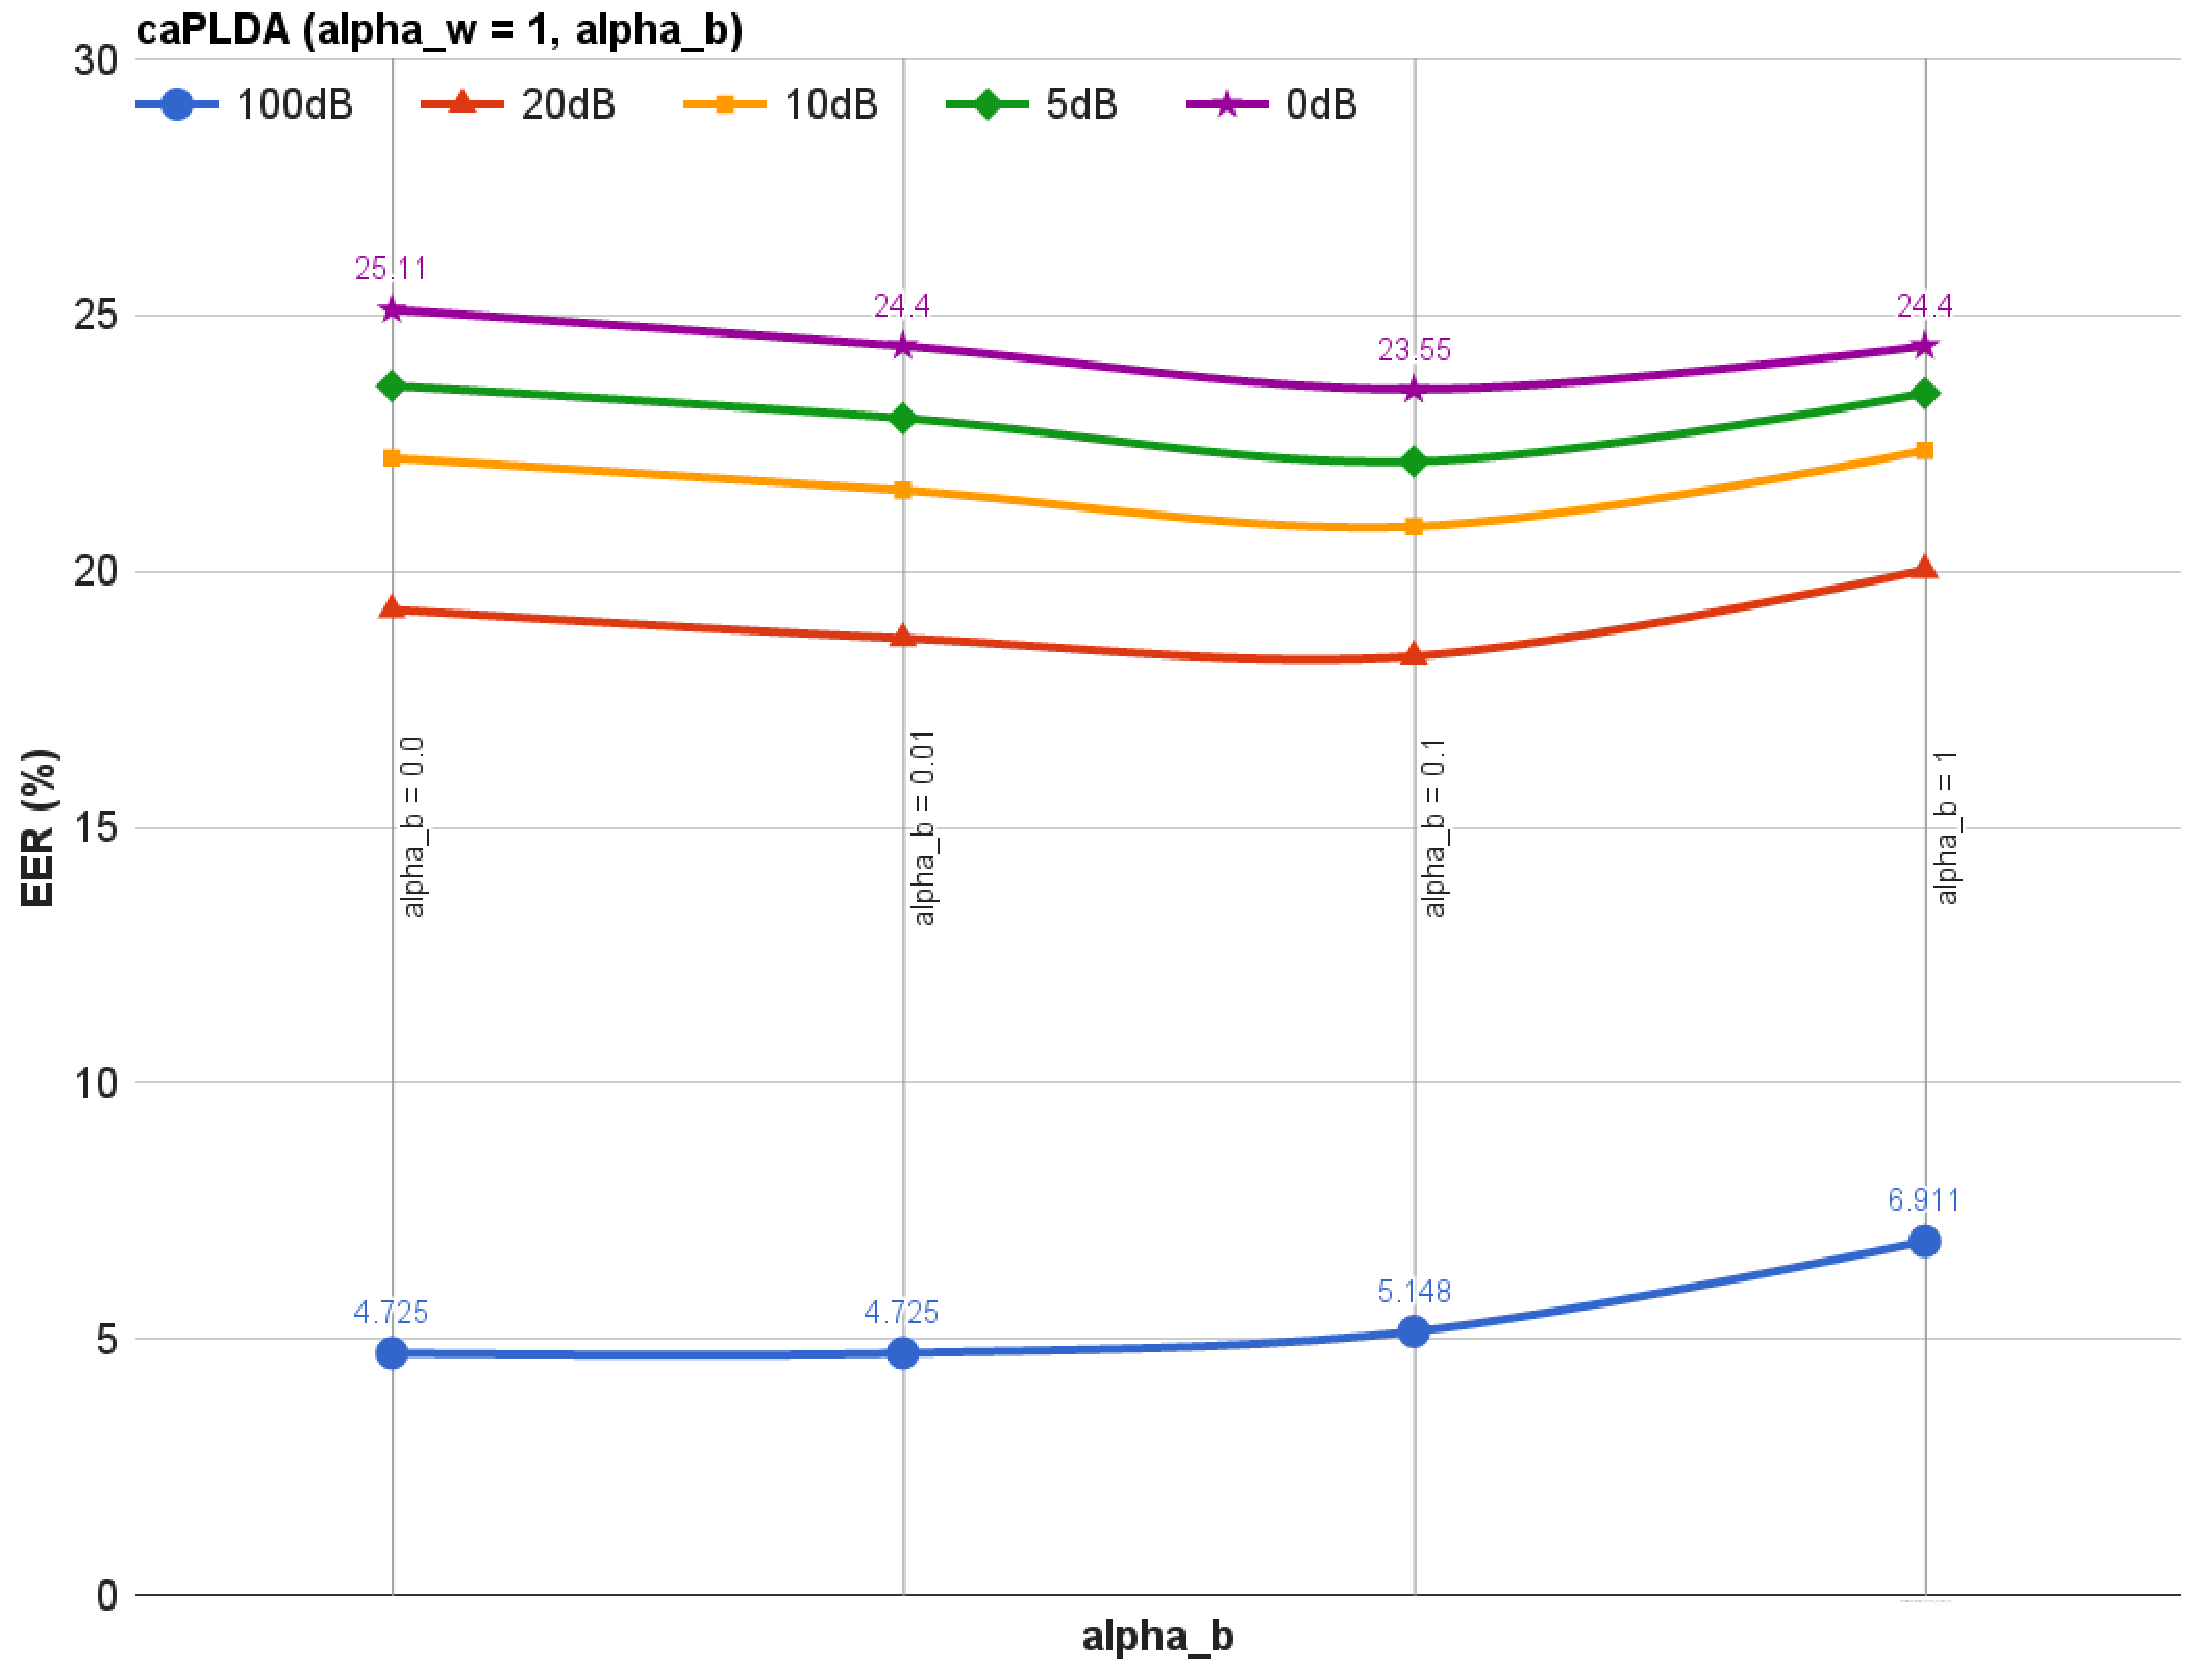
\includegraphics[height = 3.2in, width=0.7\textwidth]{figures/eer_vs_alphab}
	\vspace{-2mm}
	\caption{\it \small Comparing caPLDA for different values of between-speaker coefficient ($\alpha_b$). Here we set $\alpha_w$ to 1. The curves start from left with $\alpha_b = 0$, the scenario equivalent to what is shown in Fig.~\ref{fig:cch_in_sid}. The bottom (blue) lines shows the effect on clean trials, in which modifying simplified PLDA always degrades performance. For co-channel trials, however, setting $\alpha_b$ to non-zero values improves performance for all SIR values.}
	\label{fig:alpha_w_is_1}
	\vspace{-1mm}
\end{figure*}

Our second attempt is to investigate the special case in which $\alpha_w$ is set to $0$ and $\alpha_b=1$, as proposed in Sect.~\ref{ssec:alpha_w_0}. 
We argued that in this scenario the estimate for $\Phi_b$ is likely to be most accurate. 
Table~\ref{tbl:alpha_w_0} compares setting using the three mixed PLDA scenarios plus clean PLDA. 
From the last two columns, mixed PLDA ($0, 100dB$) and clean PLDA, we see that performances are fairly close despite the additional training data in mixed PLDA ($0,100dB$). 

\begin{table*}[h!]
	\small
	\centering
	\resizebox{\textwidth}{!}
	{
	\begin{tabular}{|l|c|c|c|c|c|c|c|c|c|c|c|}
		\hline
		\multirow{2}{*}{SIR (dB)} & \multicolumn{3}{c|}{caPLDA + mixedPLDA(0dB)}          & \multicolumn{3}{c|}{caPLDA + mixedPLDA(0,5,10,20,100dB)}  & \multicolumn{3}{c|}{caPLDA + mixedPLDA(0,100dB)}             & \multicolumn{2}{c|}{caPLDA} \\ \cline{2-12} 
		& \multicolumn{2}{r|}{EER (\%)} & minDCF         & \multicolumn{2}{c|}{EER (\%)} & minDCF             & \multicolumn{2}{c|}{EER (\%)}       & minDCF          & EER(\%)               & minDCF       \\ \hline
		100                       & \multicolumn{2}{c|}{9.03}     & 0.648          & \multicolumn{2}{c|}{7.12}     & 0.554              & \multicolumn{2}{c|}{\textbf{6.63}}  & 0.526           & \textbf{5.71}         & 0.465        \\ \hline
		20                        & \multicolumn{2}{c|}{21.16}    & 0.925          & \multicolumn{2}{c|}{18.55}    & 0.890              & \multicolumn{2}{c|}{\textbf{18.48}} & 0.884           & \textbf{18.83}        & 0.915        \\ \hline
		10                        & \multicolumn{2}{c|}{23.34}    & 0.956          & \multicolumn{2}{c|}{20.94}    & 0.940              & \multicolumn{2}{c|}{\textbf{20.52}} & 0.929           & \textbf{21.65}        & 0.953        \\ \hline
		5                         & \multicolumn{2}{c|}{24.96}    & 0.971          & \multicolumn{2}{c|}{22.21}    & 0.957              & \multicolumn{2}{c|}{\textbf{22.00}} & 0.951           & \textbf{22.57}        & 0.975        \\ \hline
		0                         & \multicolumn{2}{c|}{26.09}    & 0.983          & \multicolumn{2}{c|}{23.62}    & 0.978              & \multicolumn{2}{c|}{\textbf{23.06}} & 0.970           & \textbf{23.70}        & 0.986        \\ \hline
	\end{tabular}
	}
	\caption{caPLDA ($\alpha_w=0$,$\alpha_b=1$) using different co-channel training conditions. The last column show performance without co-channel data in PLDA training.}
	\label{tbl:alpha_w_0}
\end{table*}



